\subsection*{Partie I. Parties entières}
\begin{enumerate}
 \item Comme la fonction partie entière est constante sur des intervalles, il est clair que la fonction $\varphi$ le sera aussi. Les bornes de ces intervalles seront précisées plus loin. Pourtant elle ne peut être ni ni en escalier ni continue par morceaux (ou intégrable puisque c'est la même chose) car son domaine de définition n'est pas un segment. En revanche, la restriction $\varphi_m$ est en escalier donc continue par morceaux et intégrable.
 \item
\begin{enumerate}
 \item Pour tout $x>0$, on écrit les définitions des deux parties entières et on combine les encadrements
\begin{multline*}
 \left. 
\begin{aligned}
 &\frac{2}{x}-1 < \lfloor \frac{2}{x} \rfloor \leq \frac{2}{x}\\
 &\frac{1}{x}-1 < \lfloor \frac{1}{x} \rfloor \leq \frac{}{x}
\end{aligned}
\right\rbrace
\Rightarrow \frac{2}{x}-1 -2\frac{1}{x}<\varphi(x)<\frac{2}{x}-2(\frac{1}{x}-1)\\
\Rightarrow -1 <\varphi(x) <2 \Rightarrow \varphi(x)\in\{0,1\} 
\end{multline*}
car $\varphi$ est à valeurs entières.
 \item Remarquons d'abord que $\varphi$ prend la valeur $0$ en un inverse d'entier. On se place donc dans l'intervalle ouvert. D'une part, 
\begin{displaymath}
 \frac{1}{k+1}<x<\frac{1}{k}\Rightarrow k< \frac{1}{x} < k+1 \Rightarrow \lfloor \frac{1}{x} \rfloor = k
\end{displaymath}
D'autre part,
\begin{displaymath}
 \frac{1}{k+1}<x<\frac{1}{k}\Rightarrow 2k< \frac{2}{x} < 2k+2 \Rightarrow \lfloor \frac{2}{x} \rfloor \in \{ 2k,2k+1\}
\end{displaymath}
avec :
\begin{align*}
 &\varphi(x)=0\Leftrightarrow\lfloor \frac{2}{x} \rfloor=2k \Leftrightarrow \frac{2}{x}<2k+1
\Leftrightarrow x>\frac{2}{2k+1}=\frac{1}{k+\frac{1}{2}}\\
 &\varphi(x)=1 \Leftrightarrow \lfloor \frac{2}{x} \rfloor=2k+1 \Leftrightarrow \frac{2}{x}\geq 2k+1
\Leftrightarrow x \leq \frac{2}{2k+1}=\frac{1}{k+\frac{1}{2}}
\end{align*}
On en déduit le graphe présenté en figure \ref{fig:Cfesc1_1}.
\begin{figure}[h!t]
 \centering
 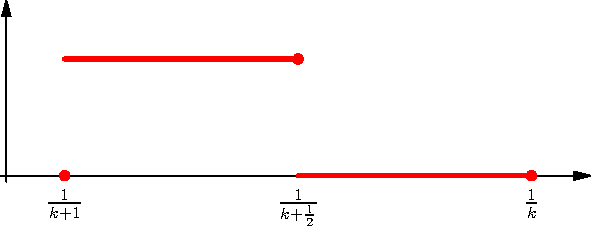
\includegraphics{Cfesc1_1.pdf}
 % Cfesc1_1.pdf: 0x0 pixel, 0dpi, 0.00x0.00 cm, bb=
 \caption{Graphe de $\varphi$ dans $\left[ \frac{1}{k+1},\frac{1}{k}\right]$}
 \label{fig:Cfesc1_1}
\end{figure}

 \item D'après les définitions,
\begin{multline*}
 k\in D_n \Leftrightarrow \frac{n}{k}-\lfloor \frac{n}{k}\rfloor \geq \frac{1}{2}
\Leftrightarrow \frac{2n}{k}-2\lfloor \frac{n}{k}\rfloor \geq 1
\Leftrightarrow \lfloor \frac{2n}{k}\rfloor +\{\frac{2n}{k}\}-2\lfloor \frac{n}{k}\rfloor \geq 1 \\
\Leftrightarrow \varphi(\frac{k}{n})\geq 1-\{\frac{2n}{k}\}
\Leftrightarrow \varphi(\frac{k}{n}) > 0 \hspace{0.5cm}\text{ (car $\{x\}\in [0,1[$)}
\Leftrightarrow \varphi(\frac{k}{n}) = 1 .
\end{multline*}
\end{enumerate}
\item On calcule l'intégrale en utilisant la relation de Chasles et le graphe de la figure \ref{fig:Cfesc1_1}
\begin{multline*}
 \int_{[\frac{1}{m},1]}\varphi = \sum_{k=1}^{m-1}\int_{[\frac{1}{k+1},\frac{1}{k}]}\varphi
= \sum_{k=1}^{m-1}\left(
         \int_{[\frac{1}{k+1},\frac{1}{k+\frac{1}{2}}]}\underset{= 1}{\underbrace{\varphi}}
        + \int_{[\frac{1}{k+\frac{1}{2}} , \frac{1}{k},]} \underset{= 0}{\underbrace{\varphi}} 
                 \right) \\
=  \sum_{k=1}^{m-1}\left(\frac{1}{k+\frac{1}{2}} - \frac{1}{k+1}\right) 
=  \sum_{k'=2}^{m}\left(\frac{1}{k'-\frac{1}{2}} - \frac{1}{k'}\right)
= \sum_{k=2}^m \frac{1}{k-\frac{1}{2}} - \sum_{k=2}^m \frac{1}{k}
\end{multline*}

\item
\begin{enumerate}
 \item On manipule l'expression obtenue pour l'intégrale en utilisant $\frac{1}{k-\frac{1}{2}}=\frac{2}{2k-1}$ et en dégageant le rôle des entiers pairs et impairs.
\begin{multline*}
\int_{[\frac{1}{m},1]}\varphi 
= 2\left(\frac{1}{3}+\frac{1}{5}+\cdots+\frac{1}{2m-1} \right) -\left(\frac{1}{2}+\frac{1}{3}+\cdots+\frac{1}{m} \right)\\
= 2\left[\left(1+\frac{1}{2}+\frac{1}{3}+\cdots+\frac{1}{2m}\right)-1 
         -\left(\frac{1}{2}+\frac{1}{4}+\cdots+\frac{1}{2m}\right)\right] \\
  - \left[\left(1+\frac{1}{2}+\frac{1}{3}+\cdots+\frac{1}{m}\right)-1 \right]\\
=2h_{2m}-2-2h_m+1 = 2h_{2m}-2h_m-1 .
\end{multline*}

 \item En utilisant le développement donné par l'énoncé, il vient
\begin{displaymath}
\int_{[\frac{1}{m},1]}\varphi =2\left[\ln(2m)-\ln(m)+o(1) \right]-1
=2\ln2 -1 +o(1)\rightarrow 2\ln2 -1 .
\end{displaymath}
\end{enumerate}
\end{enumerate}

\subsection*{Partie II. Sommes de Riemann}
\begin{enumerate}
 \item Regardons $S_n$ comme l'intégrale d'une fonction en escalier $\overline{\psi}$ formée à partir des valeurs de $\psi$. La subdivision $\overline{\mathcal S}$ définissant $\overline{\psi}$  est constituée par les extrémités $a$ et $b$ et les $\frac{k}{n}$ dans l'intervalle $[a,b]$ (tirets dans la figure \ref{fig:Cfesc1_2}).\newline
 \begin{figure}[h]
 \centering
 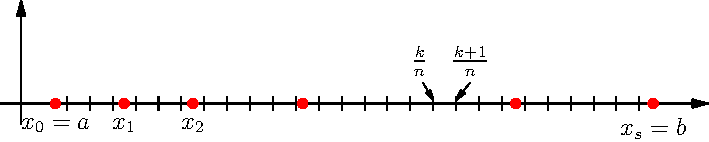
\includegraphics{Cfesc1_2.pdf}
 \caption{Subdivisions $\mathcal S$ et $\overline{\mathcal S}$}
 \label{fig:Cfesc1_2}
\end{figure}
La fonction $\overline{\psi}$ est nulle sur le premier intervalle (entre $a$ et le tiret le plus à gauche). Sur chacun des intervalles suivants, la valeur est celle de $\psi$ au tiret de gauche. Pour $\overline{\psi}$ ainsi définie, $S_n$ est bien l'intégrale de $\overline{\psi}$ entre $a$ et $b$.\newline 
D'après l'hypothèse $\frac{1}{n}<\alpha$, la longueur d'un intervalle de $\overline{\mathcal S}$ est toujours plus petite que la longueur d'un intervalle de $\mathcal S$ (figure \ref{fig:Cfesc1_2}).
La différence que l'on nous demande de majorer est la valeur absolue de l'intégrale de $\overline{\psi}-\psi$. On la découpe à l'aide de la relation de Chasles en une somme d'intégrales sur les intervalles $[\frac{k}{n},\frac{k+1}{n}]$ de $\overline{\mathcal S}$.\\ 
Considérons un intervalle (ouvert) de $\overline{\mathcal S}$.\newline
S'il ne contient aucun des $x_i$ alors $\psi$ et $\overline{\psi}$ coïncident sur cet intervalle. Sur un tel intervalle les deux intégrales sont égales.\newline
Les seuls intervalles qui contribuent réellement sont donc ceux contenant un $x_i$. Il y en a au plus $m+1$ (le nombre de $x_i$), leur longueur est au plus $\frac{1}{n}$, la différence des fonctions $\psi$ et $\overline{\psi}$ est majorée en valeur absolue par $2M$. On en déduit l'inégalité demandée.
 \item
\begin{enumerate}
 \item On a vu en I.1.c. que $\varphi(\frac{k}{n})=1$ si et seulement si $k\in D_n$ et que la valeur de $\varphi$ est nulle sinon. On en déduit que 
\begin{displaymath}
 \sharp D_n = \sum_{k=1}^n\varphi(\frac{k}{n})\Rightarrow d_n = \frac{1}{n} \sum_{k=1}^n\varphi(\frac{k}{n}).
\end{displaymath}
 
 \item Pour obtenir l'inégalité demandée, on applique l'inégalité de la question II.1. à la fonction en escalier $\varphi_m$ dans le segment $[\frac{1}{m},1]$.\newline
 Comme  $|\varphi$ est majoré par $M=1$, il reste à préciser le nombre $s+1$ de points d'une subdivision adaptée à $\varphi_m$.\newline
 D'après la question 2 de la partie I. Une subdivision adaptée est formée par les $\frac{1}{k}$ et les $\frac{1}{k+\frac{1}{2}}$ entre $\frac{1}{m}$ et $1$. 
\[
 \frac{1}{m}\leq \frac{1}{k} \leq 1 \Leftrightarrow k\in \llbracket 1,m\rrbracket, \hspace{0.5cm}
 \frac{1}{m}\leq \frac{1}{k+\frac{1}{2}} \leq 1 \Leftrightarrow k\in \llbracket 0,m-1\rrbracket.
\]
 Le nombre total (qui est le $s+1$ de l'inégalité de la question 1) de points de la subdivision adaptée à $\varphi_m$ est donc $2m$.
\end{enumerate}

 \item Notons $l=2\ln 2-1$. On va former une majoration valable pour les entiers $n>m$ (avec $m$ à priori arbitraire). On verra après comment choisir ce $m$ en fonction d'un $\varepsilon>0$ arbitraire pour valider la définition de la limite.
\begin{multline*}
 \left\vert d_n - l\right\vert
\leq \left\vert \frac{1}{n}\sum_{k\text{ tq }\frac{k}{n}<\frac{1}{m}}\varphi(\frac{k}{n})\right\vert
    + \left\vert \frac{1}{n}\sum_{k\text{ tq }\frac{k}{n}\geq\frac{1}{m}}\varphi(\frac{k}{n})
                 -\int_{[\frac{1}{m},1]}\varphi \right\vert
    +\left\vert \int_{[\frac{1}{m},1]}\varphi -l\right\vert \\
\leq \frac{1}{n}\times \frac{n}{m}\times 1 + \frac{4m}{n} + \left\vert \int_{[\frac{1}{m},1]}\varphi -l\right\vert 
\leq \frac{1}{m} + \frac{4m}{n} + \left\vert \int_{[\frac{1}{m},1]}\varphi -l\right\vert
\end{multline*}
On est alors en mesure de prouver la convergence.\\
Pour tout $\varepsilon>0$, il existe un $m$ vérifiant:
\begin{align*}
  \frac{1}{m}\leq \frac{\varepsilon}{3}
 & & \left\vert \int_{[\frac{1}{m},1]}\varphi -l\right\vert \leq \frac{\varepsilon}{3}.
\end{align*}
Ce $m$ étant fixé, la suite $\left(\frac{4m}{n}\right) _{n\in \N^*}$ converge vers $0$. Il existe donc un $N$ (que l'on prend $\geq m$) tel que
\begin{displaymath}
 n\geq N \Rightarrow \frac{4m}{n} \leq \frac{\varepsilon}{3}.
\end{displaymath}
On aura bien alors
\begin{displaymath}
 n\geq N \Rightarrow \left\vert d_n - l\right\vert \leq \varepsilon.
\end{displaymath}
\end{enumerate}
